\section{Systeem}



\subsection{Vriendjes}

De directe buren en buren die we kennen via directe buren (via's) worden opgeslagen als een `vriendje' object. Deze vriendjes worden opgeslagen in een simpele array. De array is standaard 253 vriendjes lang, aangezien dat het maximale aantal is dat er kunnen zijn volgens de ISO. In \autoref{fig:friendsList} is de werking van de vriendjes array te zien.


\begin{figure}[ht]
    \centering
    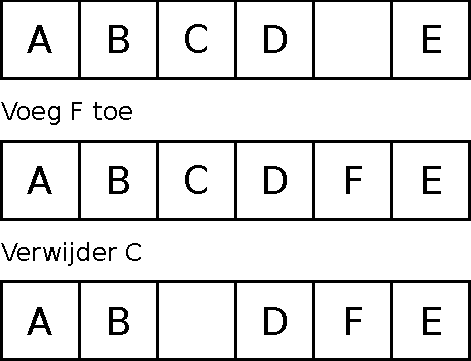
\includegraphics[width=0.45\textwidth]{img/friendList.pdf}
    \caption{Hoe de vriendjes array werkt}
    \label{fig:friendsList}
\end{figure}

De array is zo gemaakt dat, wanneer een node weggehaald moet worden, zijn ID gewoon naar 0 gezet kan worden. Wanneer het ID van een van de vriendjes in de array 0 is, wordt deze genegeerd door de code. Wanneer er een nieuw vriendje toe wordt gevoegd, word deze op de eerst mogelijke positie gezet waar het ID gelijk is aan 0. Op deze manier hoeft de array niet elke keer opgeschoven te worden wanneer er een vriendje weggehaald wordt.

Er zijn 2 soorten vriendjes: een direct vriendje en een via. Deze worden in hetzelfde datatype in dezelfde array opgeslagen. Elk vriendje bevat de volgende data:
\begin{description}
    \item[ID]       Het ID van het vriendje.
    \item[Hops]     In hoeveel hops het vriendje bekend is.
    \item[Via]      Via welk directe vriendje dit vriendje bekend is.
    \item[Trust]    Hoe goed we een direct vriendje vertrouwen.
    \item[Actief]   Of het vriendje betrouwbaar genoeg is om berichten naar te kunnen sturen.
\end{description}
